\section{Processi di supporto}

\subsection{Gestione ticket}
\label{gestioneticket}

Abbiamo ritenuto poco efficiente utilizzare la piattaforma \glossario{TeamworkPM} per la gestione sia delle attività che delle modifiche, poiché l'utilizzo che volevamo farne non sfruttava appieno le funzionalità di ``Diagramma Gantt'' e ``Task List''. È stata fatta quindi la seguente separazione:
\begin{itemize}
 \item \textbf{gestione delle attività}: viene fatta utilizzando i \glossario{task} di \glossario{TeamworkPM}
 \item \textbf{gestione delle modifiche}: viene fatta utilizzando le \glossario{issue} di \glossario{GitHub}
\end{itemize}

Quando non è specificato come modificare il valore di un parametro delle \glossario{issue} bisogna mantenere il valore già presente, o quello di default se la \glossario{issue} è appena stata creata.

\subsubsection{Richiesta di modifica e segnalazione bug}
\label{aperturaissue}

\begin{figure}[H]
    \centering
    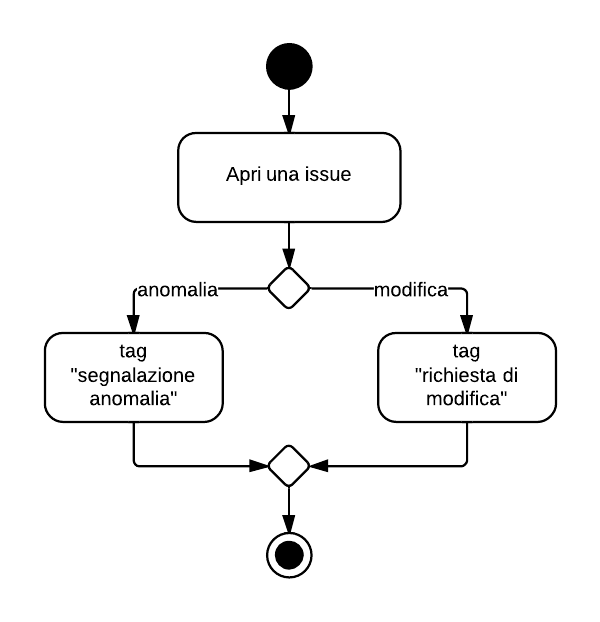
\includegraphics[width=9cm]{uml-processi/richiesta_di_modifica_e_segnalazione_bug.png}
    \caption{Richiesta di modifica e segnalazione bug}
\end{figure}

Se un membro del gruppo intende segnalare un bug o richiedere una modifica deve aprire una \glossario{issue} su \glossario{GitHub} con i seguenti parametri:
\begin{itemize}
 \item \textbf{Titolo}: un titolo breve ma descrittivo.
 \item \textbf{Descrizione}: una descrizione esaustiva dell'anomalia riscontrata o della modifica richiesta.
 \item \textbf{Tag}: uno tra i seguenti:
  \begin{itemize}
   \item \textbf{segnalazione anomalia}: da usare se si vuole segnalare un bug, un malfunzionamento, un'anomalia in genere che non dovrebbe esserci nei documenti ufficiali o nel prodotto finale;
   \item \textbf{richiesta di modifica}: da usare se si vuole richiedere al Responsabile una modifica.
  \end{itemize}
 \item \textbf{Assegnato a}: il Responsabile
 \item \textbf{Milestone}: nessuna
\end{itemize}

\subsubsection{Progettazione unità di lavoro}

\begin{figure}[H]
    \centering
    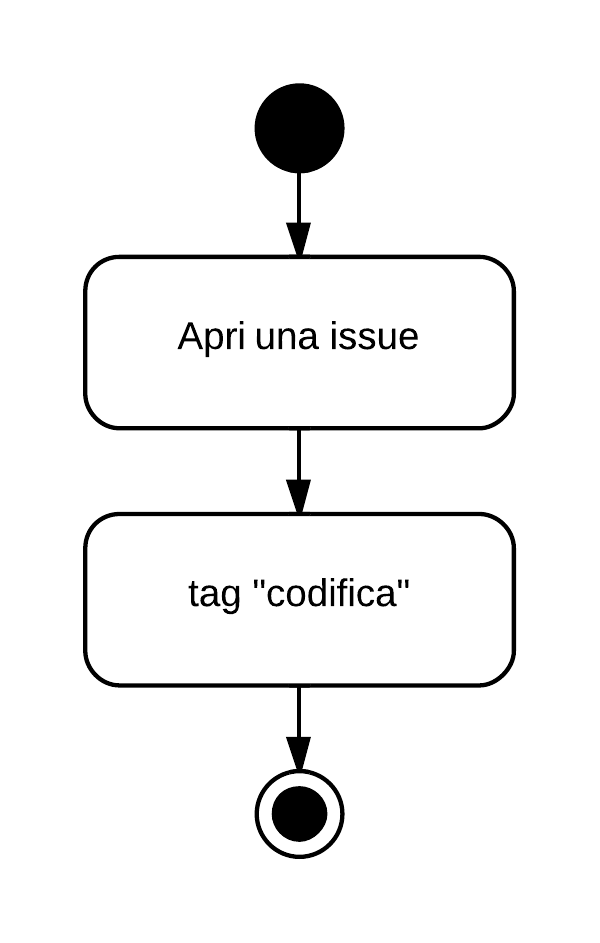
\includegraphics[height=7cm]{uml-processi/progettazione_unita_di_lavoro.png}
    \caption{Creazione compito}
\end{figure}

Il Progettista, dopo aver completata la progettazione di dettaglio, deve creare le \glossario{issue} di codifica con i seguenti parametri:
\begin{itemize}
 \item \textbf{Titolo}: un titolo breve ma descrittivo.
 \item \textbf{Descrizione}: una descrizione esaustiva dell'attività da svolgere, con tutti i riferimenti necessari.
 \item \textbf{Tag}: \textbf{codifica}
 \item \textbf{Assegnato a}: il Responsabile
 \item \textbf{Milestone}: nessuna
\end{itemize}

\subsubsection{Valutazione issue}

\begin{figure}[H]
    \centering
    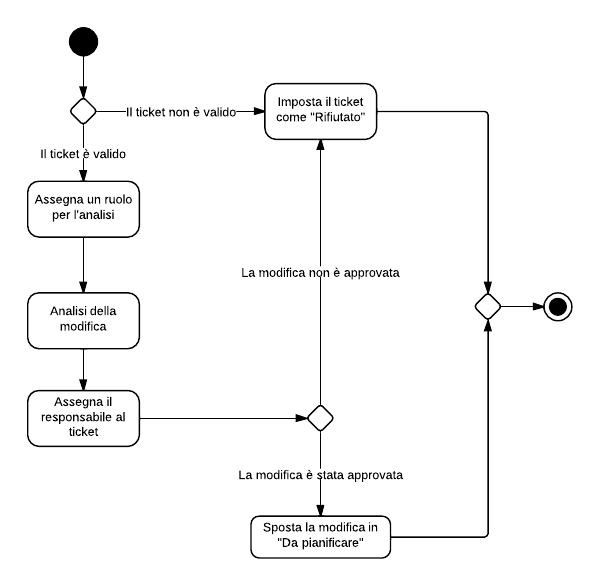
\includegraphics[width=\textwidth]{uml-processi/valutazione_issue.png}
    \caption{Valutazione issue}
\end{figure}

Il Responsabile deve valutare ogni nuova \glossario{issue}. Se ritiene che la formulazione sia corretta e se è necessario approfondire la modalità in cui verrà eseguita l'attività richiesta, allora il Responsabile deve anche assegnare la \glossario{issue} ad un ruolo competente:
\begin{itemize}
 \item \textbf{Assegnato a}: un ruolo a scelta del Responsabile
\end{itemize}

Tale ruolo, dopo averla analizzata, deve riassegnarla al Responsabile aggiungendo le informazione prodotte dall'analisi:
\begin{itemize}
 \item \textbf{Assegnato a}: il Responsabile
 \item \textbf{Descrizione}: la descrizione già presente con in aggiunta i risultati dell'analisi.
\end{itemize}

A questo punto, se il Responsabile ritiene che l'attività debba essere eseguita, pianifica la issue secondo la procedura \ref{pianificazione}.

Se il Responsabile non approva o non ritene valida la \glossario{issue} deve chiuderla impostando:
\begin{itemize}
 \item \textbf{Tag}: uno tra i seguenti
  \begin{itemize}
   \item \textbf{scritto male}: se la descrizione o il titolo sono poco comprensibili;
   \item \textbf{non lo faremo}: se ritiene che non valga la pena si svolgere l'attività richiesta;
   \item \textbf{duplicato}: se l'attività è già stata richiesta da un'altra \glossario{issue}. In questo caso è raccomandabile aggiungere nella descrizione un riferimento alla \glossario{issue} originale.
  \end{itemize}
 \item \textbf{Stato}: ``Chiuso''.
\end{itemize}

\subsubsection{Pianificazione issue}
\label{pianificazione}

\begin{figure}[H]
    \centering
    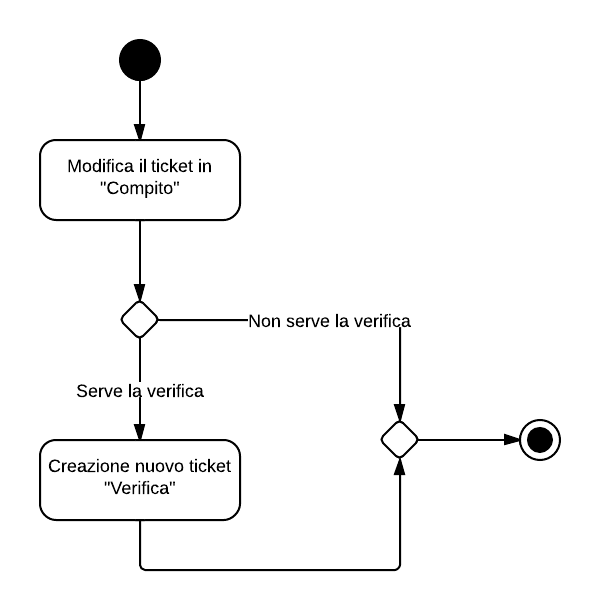
\includegraphics[width=12cm]{uml-processi/pianificazione_issue.png}
    \caption{Pianificazione issue}
\end{figure}

Il Responsabile deve pianificare le \glossario{issue} a lui assegnate e marcate ``approvato'' o ``codifica'' creando un \glossario{task}. Deve inoltre pianificare il corrispondente \glossario{task} di verifica se necessario. I \glossario{task} del compito e della modifica devono essere assegnati a persone diverse.

Modifica i parametri della \glossario{issue}:
\begin{itemize}
 \item \textbf{Assegnato a}: nessuno.
\end{itemize}

Se esiste già un \glossario{task} a cui associare la \glossario{issue} il Responsabile deve scegliere una delle seguenti opzioni:
\begin{itemize}
 \item modificare tale \glossario{task} con questi parametri:
	\begin{itemize}
		\item \textbf{Descrizione}: la descrizione precedente, con in aggiunta un riferimento evidente alla \glossario{issue}.
	\end{itemize}
 \item creare un \glossario{task} secondario (``subtask'' nel gergo di TeamworkPM) con i seguenti parametri:
	\begin{itemize}
		\item \textbf{Titolo}: un titolo breve ma descrittivo, magari simile a quello della \glossario{issue}.
		\item \textbf{Descrizione}: una breve descrizione, con un riferimento evidente alla \glossario{issue}.
		\item \textbf{Assegnato a}: la stessa persona a cui è associato il \glossario{task} principale.
	\end{itemize}
\end{itemize}

Se il \glossario{task} non esiste, allora deve crearne uno nuovo seguendo la procedura \ref{creazionetask}.

Analogamente, se esiste già un \glossario{task} a cui associare la verifica, il Responsabile deve scegliere una delle seguenti opzioni:
\begin{itemize}
 \item modificare tale \glossario{task} di verifica con questi parametri:
	\begin{itemize}
		\item \textbf{Descrizione}: la descrizione precedente, con in aggiunta un riferimento evidente al \glossario{task} da verificare.
	\end{itemize}
 \item creare un \glossario{task} secondario (``subtask'' nel gergo di TeamworkPM) con i seguenti parametri:
	\begin{itemize}
		\item \textbf{Titolo}: un titolo breve ma descrittivo, magari simile a quello della \glossario{issue}.
		\item \textbf{Descrizione}: una breve descrizione, con un riferimento evidente alla \glossario{issue}.
		\item \textbf{Assegnato a}: la stessa persona a cui è associato il \glossario{task} principale.
	\end{itemize}
\end{itemize}

Se il \glossario{task} di verifica non esiste, allora deve crearne uno nuovo seguendo la procedura \ref{creazionetask}.

\subsubsection{Creazione task}
\label{creazionetask}

\begin{figure}[H]
    \centering
    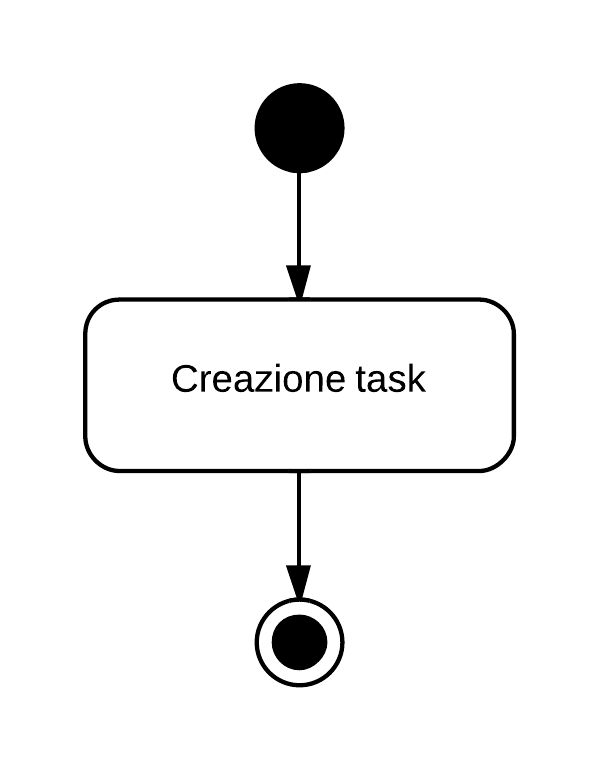
\includegraphics[height=6cm]{uml-processi/creazione_task.png}
    \caption{Creazione task}
\end{figure}

Il Responsabile può creare \glossario{task} con i seguenti parametri:
\begin{itemize}
 \item \textbf{Titolo}: il titolo dell'attività nel formato ``\{identificativo\} - \{titolo\} (\{ruolo\})'', dove
	\begin{itemize}
		\item \textbf{identificativo}: il codice che identifica l'attività nel \emph{Piano di progetto}, se presente;
		\item \textbf{titolo}: il titolo, breve e descrittivo, dell'attività.
		\item \textbf{ruolo}: il ruolo a cui è assegnato il \glossario{task}
	\end{itemize}
 \item \textbf{Assegnato a}: un membro del gruppo a scelta del Responsabile.
 \item \textbf{Pianificazione}: a scelta del Responsabile.
 \item \textbf{Descrizione}: una descrizione dell'attività (raccomandata).
 \item \textbf{Dipendenze}: i \glossario{task} di cui bisogna attendere il termine prima di poter svolgere questo \glossario{task}. In particolare, i \glossario{task} di verifica devono sempre dipendere dai \glossario{task} che devono verificare.
\end{itemize}

Solo il Responsabile può creare nuovi task.

\subsubsection{Esecuzione compito}

\begin{figure}[H]
    \centering
    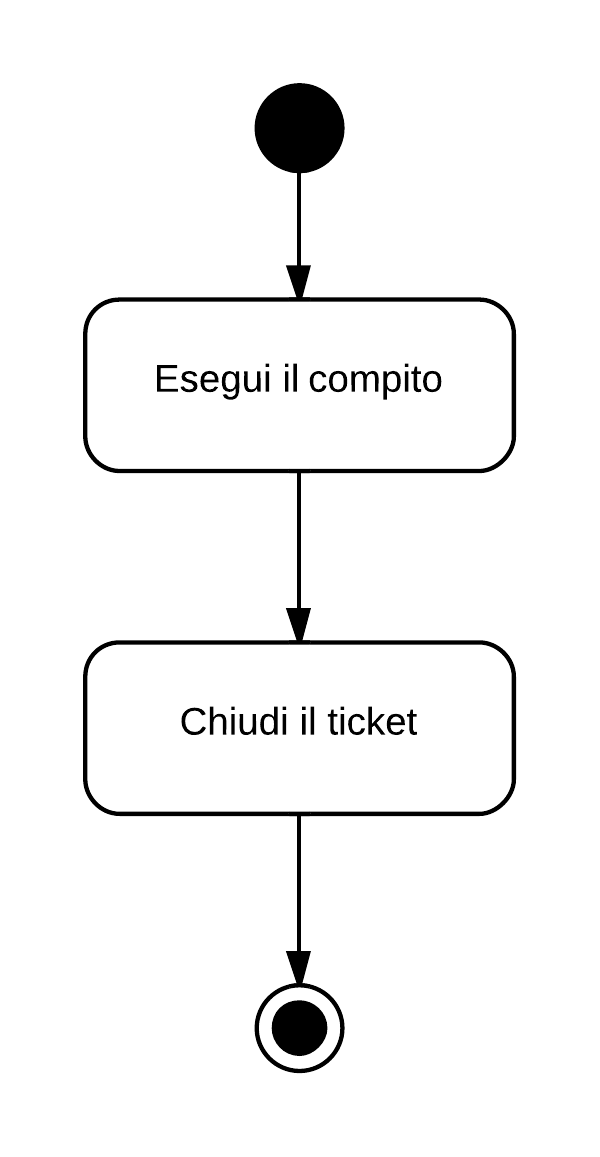
\includegraphics[width=11cm]{uml-processi/esecuzione_compito.png}
    \caption{Esecuzione compito}
\end{figure}

Il ruolo a cui è assegnato un \glossario{task} non di verifica, dopo aver svolto l'attività richiesta, deve chiudere il \glossario{task}:
\begin{itemize}
 \item \textbf{Stato task}: ``Chiuso''.
 \item \textbf{Funzione ``timer''}: registrare le ore di lavoro produttivo che sono state necessarie per completare l'attività. (Attenzione: non bisogna modificare, invece, il tempo stimato)
\end{itemize}

Inoltre deve chiudere ogni eventuale \glossario{issue} aperta associata:
\begin{itemize}
 \item \textbf{Stato issue}: ``Chiuso''.
\end{itemize}

\subsubsection{Esecuzione verifica}

\begin{figure}[H]
    \centering
    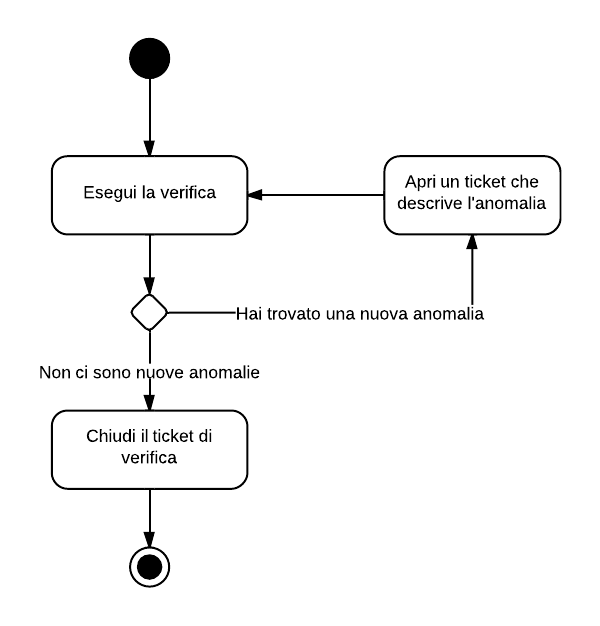
\includegraphics[width=10cm]{uml-processi/esecuzione_verifica.png}
    \caption{Esecuzione verifica}
\end{figure}

Il verificatore a cui è assegnato un \glossario{task}, dopo aver svolto l'attività richiesta, deve chiudere il \glossario{task}:
\begin{itemize}
 \item \textbf{Stato}: ``Chiuso''.
 \item \textbf{Funzione ``timer''}: registrare le ore di lavoro produttivo che sono state necessarie per completare l'attività. (Attenzione: non bisogna modificare, invece, il tempo stimato)
\end{itemize}

Nel caso in cui il verificatore trovi bug o non conformità significative deve creare una \glossario{issue}, seguendo la procedura descritta nella sezione \ref{aperturaissue}.

\subsection{Rotazione dei ruoli}
\label{rotazioneruoli}
Durante lo sviluppo del progetto vi sono diversi ruoli che ogni membro del gruppo \GroupName{} è tenuto a ricoprire almeno una volta. Per evitare possibili conflitti causati dalla rotazione dei ruoli, le attività principali assegnabili a specifici ruoli sono pianificate nel \PianoDiProgetto. Ogni componente del gruppo è tenuto a svolgere le attività assegnategli e a rispettare il ruolo che ne consegue. Il \textit{Responsabile} di progetto ha il compito di fare rispettare i ruoli assegnati durante le attività, mentre il \textit{Verificatore} deve individuare le possibili incongruenze tra i ruoli e le modifiche registrate nei diari delle modifiche.
Le incongruenze possono essere di due tipi:
\begin{itemize}
\item Il compito svolto non fa parte dei compiti propri di un dato ruolo;
\item La stessa persona verifica ciò che ha precedentemente prodotto.
\end{itemize}

Inoltre, si raccomanda che:
\begin{itemize}
\item Una persona non impieghi più del 50\% delle ore di lavoro in un unico ruolo;
\item Sia assegnato un solo task al giorno per persona.
\item I ruoli vengano ruotati ogni settimana, ma si lascia libertà al \textit{Responsabile} di ruotare in base alle esigenze.
\end{itemize}

Si predilige dunque una maggior frequenza di rotazione a discapito dell'efficienza.

Il responsabile quando assegna un ticket, come indicato nella sezione \ref{teamwork} dovrà indicare il ruolo che il destinatario ricopre nell'adempiere tale task. Questo è necessario per il diario delle modifiche dei singoli documenti e per il rendiconto economico. I ruoli sono assegnati basandosi sul \PianoDiProgetto. 

Deve inoltre tener conto delle non disponibilità a lavorare come indicato nella sezione \ref{Calendario condiviso}. \\
A supporto di tali raccomandazioni si automatizzano le verifiche utilizzando alcune funzionalità predisposte dallo script descritto nella sezione \ref{Gantt}.
	\subsubsection{Amministratore}
	
	L'\textit{Amministratore} equipaggia, organizza e gestisce l'ambiente di lavoro e di produzione. Collabora con il \textit{Responsabile} alla stesura del \textit{Piano di Progetto} e redige le \textit{Norme di Progetto}.
	Le responsabilità assunte dall'\textit{Amministratore} sono:

	\begin{itemize}

		\item Attuare le scelte tecnologiche concordate con il \textit{Responsabile} di progetto;
		\item Gestire le liste di distribuzione e assicurarne il rispetto;
		\item Controllare versioni e configurazioni del prodotto;
		\item Risolvere i problemi legati alla gestione dei processi.

	\end{itemize}

	\subsubsection{Analista}

	L'\textit{Analista} è responsabile dell'attività di analisi, pertanto deve comprendere appieno il dominio applicativo. Redige lo \textit{Studio di Fattibilità} e l'\textit{Analisi dei Requisiti} ovvero una specifica di progetto ad alto livello con vincoli e rischi tecnologici, affrontabile dal proponente, dal committente e dal \textit{Progettista}.


	\subsubsection{Progettista}

	Il \textit{Progettista} è responsabile dell'attività di progettazione, ha una profonda conoscenza dello stack tecnologico utilizzato e competenze tecniche aggiornate. Grazie a tali caratteristiche, ha una forte influenza sugli aspetti tecnici e tecnologici del progetto, e spesso ne assume responsabilità di scelta e gestione.


	\subsubsection{Programmatore}

	Il \textit{Programmatore} ha responsabilità circoscritte, si occupa dell'attività di codifica, nel rispetto delle \textit{Norme di Progetto}, miranti alla realizzazione del prodotto e delle componenti di ausilio necessarie per l'esecuzione delle prove di verifica e validazione.


	\subsubsection{Responsabile}
	
	Il \textit{Responsabile} ha l'ultima voce in capitolo per quanto concerne le decisioni sul progetto, è il responsabile ultimo dei risultati, infatti approva l'emissione dei documenti. Inoltre, redige il \textit{Piano di Progetto} assieme all'\textit{Amministratore}. 
	Le responsabilità assunte dal \textit{Responsabile} sono:

	\begin{itemize}

		\item Pianificazione e organizzazione dello sviluppo del progetto, stima tempi e costi, e assegnazione delle attività ai componenti del gruppo;
		\item Riportare lo stato del progetto ai committenti;
		\item Analizzare i rischi che possono incorrere, monitorarli e prendere provvedimenti a riguardo;
		\item Stabilire una \textit{ways of working} per ogni componente del gruppo, ai fini di un'influenza positiva delle performance del gruppo.
	
	\end{itemize}

	
	\subsubsection{Verificatore}

	Il \textit{Verificatore} organizza ed attua le attività di verifica e controlla che le attività siano conformi alle norme. Redige la parte del \textit{Piano di Qualifica} che documenta le attività svolte e i risultati ottenuti, confrontandoli con le metriche espresse nel \PianoDiQualifica. \\ 
	Le ore assegnate al verificatore devono corrispondere almeno al 30$\%$ delle ore totali suddivise tra ruoli.
	
	\subsection{Processo di Coordinamento}


\subsubsection{Comunicazioni interne}
\label{Comunicazioniinterne}

Tutte le comunicazioni ad uso interno del gruppo avvengono tramite il servizio di messaggistica offerto da \emph{TeamworkPM}, altre vie di comunicazione sono sconsigliate.

Nel caso sia necessario comunicare in modo rapido possono essere utilizzati strumenti di messaggistica istantanea come Hangouts o Skype. L'utilizzo di \glossario{SMS} e di chiamate telefoniche è riservato alle situazioni di urgenza.

\paragraph{Messaggi}
\label{Comunicazioniinternemessaggi}

\begin{itemize}
\item L'\textbf{oggetto} deve essere sintetico e coerente con il contenuto del messaggio;
\item Il \textbf{contenuto} deve includere i dettagli necessari per una corretta comprensione del messaggio e non deve essere prolisso. Il mittente può servirsi del supporto al linguaggio di \glossario{Markdown} disponibile sulla piattaforma per rendere più chiaro il suo messaggio;
\item La \textbf{categoria} deve essere coerente con l'argomento trattato. Può essere creata una categoria nuova se ritenuto necessario;
\item La \textbf{notifica} via mail deve includere gli interessati al messaggio;
\item Il livello di \textbf{privacy} deve sempre essere "\textit{Everybody on project}" in modo da permettere a tutti i componenti del gruppo di intervenire;
\item Data l'esigua dimensione dello \glossario{storage} che offre la piattaforma nella versione \textit{free} utilizzata dal gruppo e l'assenza di visualizzatori online integrati, il numero e la dimensione degli \textbf{allegati} devono essere ridotti quanto più possibile.
\end{itemize}

\paragraph{Procedura per commenti a tasks o sub-tasks}

Per tali comunicazioni valgono le regole del paragrafo \ref{Comunicazioniinternemessaggi}. Il contenuto del commento deve riguardare la task che riferisce. Se la discussione si sviluppa in argomenti non più coerenti, i componenti del gruppo \GroupName{} devono terminare la discussione, aprire un messaggio secondo le norme descritte al paragrafo \ref{Comunicazioniinternemessaggi} e inserire come nuovo commento alla discussione interrotta il link al messaggio creato con l'aggiunta della segnatura ``[OT]''. Questo non vincola il proseguimento della discussione sulla task secondo le norme.

\subsubsection{Comunicazioni esterne}
\label{email}

Le comunicazioni esterne sono gestite esclusivamente dal Responsabile di Progetto. A tal fine è stato creato l'indirizzo di posta elettronica
\begin{center} \GroupEmail{} \end{center}

Il Responsabile di Progetto si fa dunque carico di notificare ai restanti membri del gruppo eventuali corrispondenze
intrattenute con committenti e proponenti, applicando le norme stabilite al paragrafo \ref{Comunicazioniinterne}.


\subsubsection{Riunioni}

Qualora fosse necessaria una riunione di tutti o alcuni membri del gruppo sarà compito del Responsabile di Progetto avvisare gli interessati, tramite le procedure stabilite al paragrafo \ref{Comunicazioniinterne}.
Il Responsabile di Progetto decide inoltre luogo, date e ora della riunione in base al calendario a sua disposizione. Nel caso in cui qualche membro non risponda entro 24 ore il Responsabile di Progetto dovrà accertarsi con mezzi di comunicazione adeguati che tutti siano stati informati.

Ad ogni riunione verrà prodotto un verbale redatto da un segretario, ruolo svolto a turno da ogni membro del gruppo e deciso di volta in volta dal Responsabile di Progetto. Tale verbale, descritto nel paragrafo \ref{verbale} dovrà essere reso disponibile per la consultazione a tutti i membri del gruppo.

È inoltre presente un \glossario{facilitatore}, ruolo svolto a turno da ogni membro del gruppo e deciso di volta in volta dal Responsabile di Progetto, che aiuterà a rispettare l'ordine del giorno senza prolungare eccessivamente la riunione.


\subsection{Revisioni di progetto}
La vita di questo progetto didattico attraversa le revisioni di progetto specificate in \PianoDiProgetto{}, esse consistono in \emph{review}(informali) e \emph{audit} (formali) ma le modalità con cui vengono affrontate sono, da parte del gruppo, le medesime, verranno quindi in seguito denominate presentazioni o revisioni. Vengono qui descritte le procedure per le revisioni secondo quanto descritto in IEEE 1028:
\begin{enumerate}
	\setcounter{enumi}{-1}
	\item Entry evaluation: il Responsabile di Progetto prepara una checklist e si assicura che esistano le condizioni che permettano il successo della presentazione;
	\item Management preparation: il Responsabile si assicura che tutti i membri del gruppo possano partecipare e l'ambiente di lavoro rispetti i vincoli imposti o suggeriti dal committente. A tal fine è stato elaborata una lista di indicazioni (\ref{presentazione});
	\item Planning the review: il Responsabile deve identificare e confermare gli obiettivi della revisione, inoltre si assicura che tutto il team sia equipaggiato con le risorse necessarie per affrontare la revisione;
	\item Overview of review procedures: ci si assicura che tutti i membri del gruppo conoscano gli obiettivi, le procedure e il materiale portato in revisione;
	\item Individual preparation: ogni membro del gruppo si prepara individualmente per la presentazione;
	\item Group examination: il gruppo si incontra al completo e prova la presentazione confermando il rispetto dei tempi e degli obiettivi;
	\item Rework/follow-up: vengono corretti, laddove possibile,  gli errori e/o i difetti;
	\item Exit evaluation: il Responsabile si assicura che tutti gli output prodotti siano pronti per la revisione.
\end{enumerate}

\label{presentazione}
Le indicazioni su come costruire una presentazione sono le seguenti:
\begin{itemize}
	\item le diapositive devono avere la stessa densità: il rapporto tra testo, immagini e spazio vuoto deve essere uniforme;
	\item evitare testi troppo lunghi, immagini piccole o troppo dettagliate;
	\item non va spiegata la sola teoria: argomentare come è stata implementata nel progetto;
	\item la lettura delle slide deve avvenire rivolgendosi al pubblico e non rivolti verso la diapositiva; si può usare con parsimonia lo schermo del portatile per avere un riferimento;
	\item non ripetere quanto scritto nelle diapositive, è inutile;
	\item il passaggio da una diapositiva all'altra deve avvenire  tra un tempo minimo e uno massimo in modo da consentirne la lettura e non annoiare chi ascolta;
	\item le mani non devono stare nelle tasche;
	\item ogni slide deve riportare il proprio numero sul totale delle diapositive.
\end{itemize}






\subsection{Procedure per la gestione della Repository}

Come repository è stato scelto Git, in particolare il servizio \glossario{GitHub} come indicato nel capitolo \ref{github}.

\subsubsection{Repository dei documenti}

\paragraph{Struttura del repository}

La struttura del repository, la cui cartella principale chiameremo \file{root}, è così composta:
\begin{itemize}
 \item \textbf{\file{root/ufficiali/}} \\
	Contiene i documenti ufficiali approvati dal Responsabile di progetto.

 \item \textbf{\file{root/modello/}} \\
	Contiene i file comuni a due o più documenti.

 \item \textbf{\file{root/documenti/\{NomeDelDocumento\}/}} \\
	Ciascuna cartella descritta da questo percorso contiene i file che vengono utilizzati dal documento \file{\{NomeDelDocumento\}}. In particolare conterrà il file \file{\{NomeDelDocumento\}.pdf} e il file \file{diario\_ modifiche.tex}, contenente il diario delle modifiche del documento.
	
	Il nome della cartella \file{\{NomeDelDocumento\}} e il file \file{\{NomeDelDocumento\}.pdf} devono rispettare la convenzione \glossario{CamelCase}.

 \item \textbf{\file{root/script/}} \\
	Contiene gli script di supporto alle operazioni di verifica e compilazione dei documenti.
\end{itemize}

È raccomandato che tutti i file e le cartelle non contengano spazi nel loro nome. Non devono mai esserci due file o cartelle il cui percorso differisca soltanto per maiuscole/minuscole. Non bisogna inoltre rinominare file o cartelle modificandone soltanto il \glossario{case} di alcuni caratteri del nome.

\paragraph{Branch}

Il nome utilizzato per le \glossario{branch} del repository dovrà essere nella forma \textbf{nome-branch}, ossia con tutte le lettere minuscole e le parole separate da un trattino.

\paragraph{Script di pre-commit}

Con l'intenzione di ridurre al minimo la presenza di errori nei documenti caricati sul repository verrà utilizzato uno script di \code{pre-commit}. Lo script, attivato direttamente dal programma \code{git} nel momento in cui viene eseguito un commit, esegue in automatico i comandi \code{make test} e \code{make documents} descritti nella sezione \ref{makefile}. Se uno dei comandi fallisce il commit viene annullato e all'utente viene mostrato un messaggio di errore.

Per abilitare tale script di \code{pre-commit} è necessario creare un \glossario{link simbolico} con il seguente comando:
\begin{lstlisting}
ln -s {percorso assoluto del repository}/script/pre-commit {percorso assoluto del repository}/.git/hooks/pre-commit
\end{lstlisting}



\subsubsection{Repository del codice}

\paragraph{Struttura del repository}
	
La struttura del repository, la cui cartella principale chiameremo \file{root}, è così composta:
\begin{itemize}
 \item \textbf{\file{root/extra/}} \\
	Contiene script e file di supporto utilizzati per le attività di codifica.

 \item \textbf{\file{root/test/}} \\
	Contiene i file relativi ai test d'unità della libreria MaaP.

 \item \textbf{\file{root/lib/}} \\
	Contiene i file della libreria MaaP usata dalla Backend del progetto, posizionati in una cartella \code{lib} secondo la convenzione dei moduli di Node.js.

 \item \textbf{\file{root/node\_modules/}} \\
	Contiene le librerie richieste dalla libreria MaaP.

 \item \textbf{\file{root/lib/model/}} \\
	Contiene i file che gestiscono i dati utilizzati dall'applicazione e l'interfacciamento con il database.

 \item \textbf{\file{root/lib/model/dslmodel/}} \\
	Contiene i file che gestiscono la gestione dei file di configurazione dsl e l'interfacciamento di questi con il database.

 \item \textbf{\file{root/lib/view/}} \\
	Contiene i file che servono da template usati per visualizzare i dati all'utente.

 \item \textbf{\file{root/lib/controller/}} \\
	Contiene i file che gestiscono la logica con cui vengono elaborate le richieste inviate all'applicazione.

 \item \textbf{\file{root/lib/controller/middleware/}} \\
	Contiene i file che hanno il ruolo di middleware nel framework Express.

 \item \textbf{\file{root/lib/controller/service/}} \\
	Contiene i file che hanno il ruolo di service nel framework Express.

 \item \textbf{\file{root/lib/utils/}} \\
	Contiene i file di generica utilità, che non rientrano nella classificazione tra model, view e controller.

 \item \textbf{\file{root/scaffold/}} \\
	Contiene i file che verranno utilizzati come base di partenza (scaffold) per il progetto dello sviluppatore che utilizzerà il prodotto.

 \item \textbf{\file{root/scaffold/collections/}} \\
	Contiene i file di configurazione delle collection utilizzate dall'applicazione scaffold.

 \item \textbf{\file{root/scaffold/app/}} \\
	Contiene i file relativi al Frontend dell'applicazione scaffold.

 \item \textbf{\file{root/scaffold/app/view/}} \\
	Contiene i file statici html usati dal Frontend dell'applicazione scaffold.

 \item \textbf{\file{root/scaffold/app/style/}} \\
	Contiene i file statici di stile usati dal Frontend dell'applicazione scaffold.

 \item \textbf{\file{root/scaffold/app/scripts/}} \\
	Contiene i file dell'applicazione AngularJS usata nel Frontend.

 \item \textbf{\file{root/scaffold/app/scripts/services/}} \\
	Contiene i file dei service di AngularJS usata nel Frontend.

 \item \textbf{\file{root/scaffold/app/scripts/controllers/}} \\
	Contiene i file dei controller di AngularJS usata nel Frontend.

 \item \textbf{\file{root/scaffold/app/bower\_components/}} \\
	Contiene i file delle librerie utilizzate dal Frontend dell'applicazione scaffold.
	
 \item \textbf{\file{root/scaffold/node\_modules/}} \\
	Contiene i file delle librerie utilizzate dal Backend dell'applicazione scaffold.


\end{itemize}

È raccomandato che tutti i file e le cartelle non contengano spazi nel loro nome. Non devono mai esserci due file o cartelle il cui percorso differisca soltanto per maiuscole/minuscole. Non bisogna inoltre rinominare file o cartelle modificandone soltanto il \glossario{case} di alcuni caratteri del nome.

\paragraph{Branch}

Sono previsti due branch ufficiali:
\begin{itemize}
\item \textbf{stable}: contiene sempre una versione del codice che rispetta i controlli automatici effettuati dallo script `make test-report`, descritto alla sezione \ref{makefile-codifica}. Gli sviluppatori non devono effettuare modifiche direttamente su questo branch;

\item \textbf{master}: è il branch usato dagli sviluppatori per la codifica. Ad ogni commit, se il codice supera determinati test, Jenkins (descritto alla sezione \ref{jenkins}) propagherà le modifiche anche sul branch \emph{stable}.
\end{itemize}

\paragraph{Script di pre-commit}

Con l'intenzione di ridurre al minimo la presenza di errori nel codice caricato sul repository verrà utilizzato uno script di \code{pre-commit}. Lo script, attivato direttamente dal programma \code{git} nel momento in cui viene eseguito un commit, esegue in automatico il comando \code{make jshint} descritto nella sezione \ref{makefile-codifica} e controlla che non si stia facendo un commit alla branch \emph{stable}. Se il comando trova un'anomalia il commit viene annullato e all'utente viene mostrato un messaggio di errore.

Per abilitare tale script di \code{pre-commit} è necessario creare un \glossario{link simbolico} con il seguente comando:
\begin{lstlisting}
ln -s {percorso assoluto del repository}/extra/pre-commit {percorso assoluto del repository}/.git/hooks/pre-commit
\end{lstlisting}



\subsection{Condivisione file}

Per condividere internamente al gruppo dei file che non necessitano di versionamento verranno utilizzate le piattaforme:
\begin{itemize}
 \item \textbf{Google Drive} (\url{http://drive.google.com}), con l'account descritto nella sezione \ref{email};
 \item \textbf{TeamworkPM}, descritta nella sezione \ref{teamworkpm}.
\end{itemize}



\subsection{Modalità di consegna}
I documenti verranno consegnati secondo le date prestabilite dal committente e corrispondenti alle \glossario{milestone}, la modalità di consegna dovrà avvenire utilizzando \textbf{Google Drive}, creando una cartella apposita, rendendola pubblica e inviando l'email contenente il link di pubblicazione alle seguenti email: \code{tullio.vardanega@math.unipd.it}, \code{rcardin@math.unipd.it}.



\subsection{Strumenti per il coordinamento}
\label{teamworkpm}

	Per coordinare le attività, gli eventi, per le comunicazioni e per il conteggio delle ore viene utilizzata la piattaforma \textbf{Teamwork Project Manager} (\url{http://teamworkpm.net}):
	\begin{itemize}
		\item Offre un'elevata portabilità ed accessibilità essendo una piattaforma online;
		\item Offre gratuitamente i servizi necessari;
		\item Mette a disposizione delle \glossario{API} per comunicare con la piattaforma ed estenderne eventualmente le funzionalità.
	\end{itemize}
	
	L'indirizzo per accedere all'ambiente di lavoro riservato al gruppo è
	\begin{center}
		\url{https://steakholders.teamworkpm.net}
	\end{center}
	
	\subsubsection{Calendario condiviso}
	\label{Calendario condiviso}
			
	Il gruppo si avvale del calendario di Google, \glossario{Google Calendar}, come calendario condiviso.
	Tramite la propria mail personale ogni membro può accedere al calendario in modalità lettura/scrittura.
	Ogni membro è tenuto a \emph{segnalare qui i periodi di non disponibilità} nel completare i lavori assegnati, selezionando le ore o i giorni di interesse e marcandoli con la dicitura [ND], si possono aggiungere delle note se si ritiene ve ne sia necessità. 
	
	Il responsabile annoterà qui gli impegni comuni al gruppo quali riunioni ed incontri, specificando orario e luogo.
	
	\subsubsection{Strumenti per la gestione dei ticket}
	\label{teamwork}
	Per la gestione dei ticket si utilizzerà il sistema di task offerto da \glossario{TeamworkPM}, utilizzabile unicamente attraverso le procedure descritte nella sezione \ref{gestioneticket}.
	
	\subsubsection{Strumenti per la gestione del piano di lavoro}
	
	Al fine di pianificare le attività da svolgere per lo sviluppo del progetto, il gruppo si è affidato alla piattaforma \glossario{TeamworkPM} per i seguenti motivi:
	\begin{itemize}
		\item Genera automaticamente un grafico \glossario{Gantt} che visualizza e permette di modificare i task pianificati, gestendo anche le relative dipendenze;
		\item Permette di esportare il grafico \glossario{Gantt} in un formato compatibile con \glossario{GanttProject} e \glossario{Microsoft Project};
		\item Permette di gestire le \glossario{Milestone};
		\item Permette di registrare il tempo di lavoro trascorso su ogni task.
	\end{itemize}

	\subsubsection{Gestione degli eventi}
	
	Gli eventi di interesse collettivo vengono inseriti nel calendario dall'Amministratore sempre e solo nel \emph{Calendario condiviso} descritto in \ref{Calendario condiviso}.
	
	Le tipologie di eventi sono:
	\begin{itemize}
		\item \textbf{Riunioni}: vanno programmate almeno con 48 ore di anticipo tenendo conto della disponibilità dei membri. Ogni evento riunione avrà un ora di inizio e fine, un luogo e la lista dei membri che hanno confermato la partecipazione. L'\emph{ordine del giorno} dovrà essere compilato nella descrizione dell'evento;
		%In futuro potremo decidere di stilare l' \emph{ordine del giorno} nel template del verbale delle riunioni.
		\item Le \textbf{Revisioni} previste dal committente;
		\item \textbf{Non disponibilità}: un membro del gruppo dichiara di non essere disponibile a svolgere attività legate al progetto. Per creare un evento di \emph{Non disponibilità} bisogna, oltre a compilare i soliti campi (titolo, descrizione, data e ora), impostare la visibilità a \emph{tutti i membri della propria azienda}, selezionare la categoria \emph{Non disponibilità} e segnare la persona interessata. In questo modo tutti i membri del gruppo \GroupName{} potranno visualizzare tale evento. 
		Il titolo sarà nel formato \textbf{[ND] \{nome membro\}} ossia le iniziali di \emph{Non disponibilità} racchiuse tra parentesi quadre, seguite da il nome del membro del gruppo. Questo formato permetterà di individuare con immediatezza i giorni nei quali non è possibile fissare delle riunioni.
	\end{itemize}